\documentclass{beamer}

\usepackage{fancyvrb}
\usepackage{color}
\usepackage{colortbl}
\usepackage{url}

\usetheme{Singapore}
\usecolortheme{crane}

% Gets rid of PDF navigation area.
\mode<presentation>{\setbeamertemplate{navigation symbols}{}}
\setbeamercolor{snip}{fg=black,bg=craneorange!35!bg}

\title{Compile-time Typechecking\\for Custom Java Type Qualifiers}
\author{Matt Papi, Michael Ernst\\MIT CSAIL}
\date{October 22, 2007}

\begin{document}

\frame{\titlepage}

\frame
{
  \begin{center}
  {\bf\large Example:} \\ NonNull typechecker
  \end{center}
}

\frame
{
  \frametitle{Benefits of custom type qualifiers for Java}

  Type qualifiers can:
  \begin{itemize}
  \item guarantee the absence of certain errors
  \item help programmers find bugs
  \item provide clear, checkable documentation
  \item eliminate assertions and run-time checks
  \end{itemize}
}

\frame
{
  \frametitle{The demo}

  We will demonstrate the process of finding and fixing bugs using three
  typecheckers:
  \begin{itemize}
  \item NonNull/Nullable
  \item Interned
  \item Javari (ReadOnly)
  \end{itemize}
}

\setlength{\tabcolsep}{1.5\tabcolsep}
\frame
{
  \frametitle{NonNull subject programs}

  The examples I am showing come from 3 real programs:

  \begin{block}{}
  \begin{tabular}{l|c|c|c}
  \textbf{Program} & 
    \textbf{Lines} & 
    \textbf{Annotations} & 
    \textbf{Bugs found} \\ \hline
  Lookup              & 3961 & 83 & 7 \\ \hline
  NonNull checker     & 1031 & 65 & 5 \\ \hline
  Checkers framework  & 5451 & 308 & 29 
  \end{tabular}
  \end{block}
}

\frame
{
  \begin{center}
  {\bf\large Examples:} \\ Lookup, checkers framework
  \end{center}
}

% IDE: NN example #2: utilMDE.Options.jdoc/find_class_doc
% slide?: lesson learned from this example

% IDE: NN example #3: checkers.types.AnnotationUtils.findDefaultLocations
% slide?: lesson learned from this example

% IDE: NN example #4: checkers.nonnull.NonNullAnnotatedTypeFactory
% slide? lesson learned from this example

\setlength{\tabcolsep}{2.7\tabcolsep}
\frame
{
  \frametitle{Comparison with other tools: Lookup}

  \begin{center}
  Lookup contained 7 null-related bugs.
  \end{center}

  \begin{block}{}
  \begin{tabular}{l|c|c}
  \textbf{Tool} & \textbf{Warnings} & \textbf{Errors} \\ \hline
  Our typechecker & 0 & 7 \\ \hline
  FindBugs & 1 & 0 \\ \hline
  JLint & 0 & 0 
  \end{tabular}
  \end{block}{}
}

\frame
{
  \frametitle{Interning}
  \begin{itemize}
  \item Also known as canonicalization or hash-consing
  \item A space optimization: reuse an existing object instead of creating a new one
  \begin{itemize}
  \item The space savings can be significant
  \end{itemize}
  \item Built into \texttt{java.lang.String}: \texttt{intern()} method
  \only<1>{
      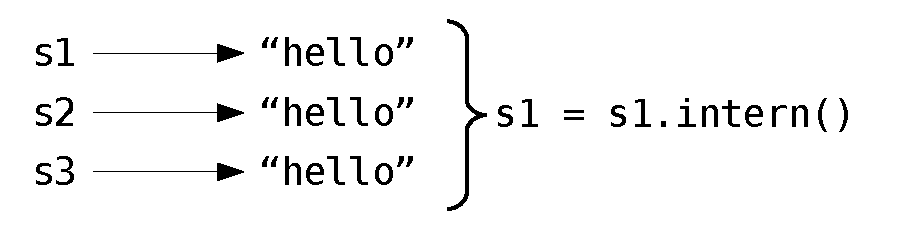
\includegraphics[height=5.0em]{interned-fig/interned-fig-1.pdf}
  }
  \only<2>{
      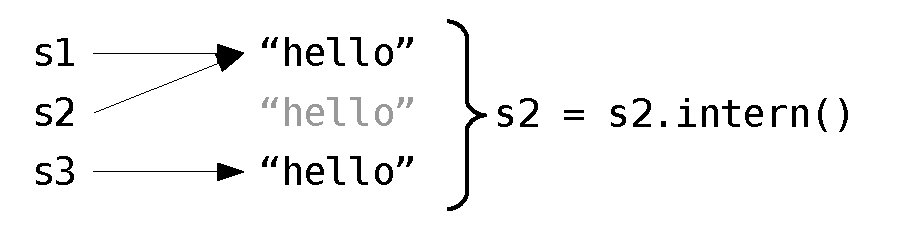
\includegraphics[height=5.0em]{interned-fig/interned-fig-2.pdf}
  }
  \only<3>{
      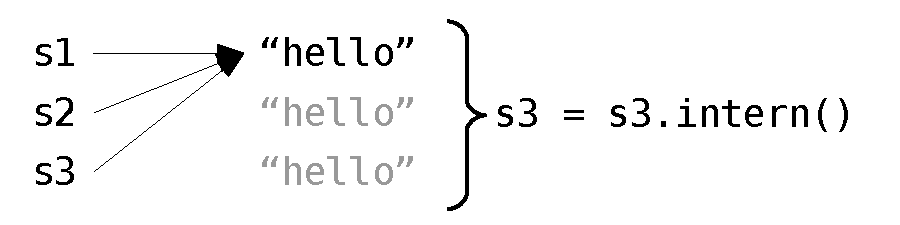
\includegraphics[height=5.0em]{interned-fig/interned-fig-3.pdf}
  }
  \item Users can add interning for their own classes
  \end{itemize}
}

\frame
{
  \frametitle{Interning (2)}

  \begin{itemize}
  \item Interning also saves time: can compare with \texttt{==}

  \VerbatimInput[fontsize=\footnotesize]{snippet-interned1.java}

  \item Potential for error: using \texttt{==} on non-interned objects

  \VerbatimInput[fontsize=\footnotesize]{snippet-interned2.java}

  \item Benefits of automatic checking:

  \begin{itemize}
  \item guarantee that no space savings were overlooked
  \item guarantee of no equality-checking errors
  \end{itemize}

  \end{itemize}
}

\frame
{
  \frametitle{Daikon invariant detector}
  \begin{itemize}
  \item Memory is the limiting factor in scaleability
  \item Daikon makes extensive use of space optimizations such as interning
  \item 250KLOC of Java code
  \item 1200 lines of code/comments about interning
  \item 200 run-time assertions checking interning
  \end{itemize}
}

\frame
{
  \frametitle{Daikon case study}

  Added to Daikon:
  \begin{itemize}
  \item 127 @Interned annotations
  \begin{itemize}
  \item Most files require no annotations
  \end{itemize}
  \item 14 @SuppressWarnings annotations
  \end{itemize}


  Results:
  \begin{itemize}
  \item Detected 9 correctness errors
  \item Detected 2 performance bugs
  \end{itemize}
}

\frame
{
  \begin{center}
  {\bf\large Examples:} \\ Daikon
  \end{center}
}

% ---

\frame
{
  \frametitle{Javari: Java with reference immutability}

  A ReadOnly reference cannot be used to modify its referent.

  \begin{center}
  \only<1>{
  \VerbatimInput[commandchars=\\\{\},fontsize=\footnotesize]{snippet-javari1.java}
  }
  \only<2>{
  \VerbatimInput[commandchars=\\\{\},fontsize=\footnotesize]{snippet-javari2.java}
  }
  \end{center} 
}

\frame
{
  \begin{center}
  {\bf\large Examples:} \\ Listmatcher, Javari checker
  \end{center}
}

\frame
{
  \frametitle{Javarifier}

  \begin{itemize}
  \item The Javarifier infers Javari annotations:

  \begin{itemize}
  \item input: a set of class files
  \item output: a set of annotated class files (or source, if available)
  \end{itemize}

  \item Useful when working with third-party libraries or legacy code
  \end{itemize}

}

% ---

\frame
{
  \frametitle{Writing annotations on types}

  \begin{itemize}
  \item Annotations on types enabled by JSR 308
  \item Backward-compatibility mode so code can compile in Java 5 and 6
  (annotations in comments: \texttt{/*@NonNull*/})
  \end{itemize}
}

\frame
{
  \frametitle{Creating new typecheckers}

  We have developed a framework for writing typecheckers:
  \begin{itemize}
  \item a template for traversing a program's source code
  \item an API for querying the annotations on types
  \item interfaces to the Java compiler (for reporting errors, querying the
        parse tree, etc.)
  \end{itemize}

  (The Interned and NonNull typecheckers are each around 350 lines of code.)

}

\frame
{
  \frametitle{Summary: Custom type qualifiers for Java}
  \begin{center}
  We have created typecheckers for NonNull, Interned,\\the Javari language,
  and the IGJ language.
  \end{center}

  Programmers can:
  \begin{itemize}
  \item write qualifiers anywhere that types are used
  \item find and prevent bugs at compile time 
  \item obtain guarantees that programs are free of certain errors
  \item create custom qualifiers and type-checkers
  \end{itemize}

  \begin{center}
  Download:\\
  \color{orange}{\Large \url{http://pag.csail.mit.edu/jsr308}}
  \end{center}
}

\end{document}

